\documentclass[../../main.tex]{subfiles}
\begin{document}

{\bf [解答]}

与えられた関数
\begin{align}
  f(x)=\int_x^{x+1}te^{-|t|}dt \label{eq:1}
\end{align}
について考える．

\paragraph{(1)}

$-1\le x\le0$の時\cref{eq:1}の絶対値を外して
\begin{align}
  f(x)=\int_x^0te^tdt+\int_0^{x+1}te^{-t}dt
\end{align}
より，両辺微分して
\begin{align}
  f'(x)
  &=-xe^x+(x+1)e^{-x-1}\\
  &=e^{-x}\left[\dfrac{1}{e}(x+1)-xe^{2x}\right]\ge0\quad(\because-1\le x\le0)
\end{align}
だから$f(x)$は単調増加で，
\begin{align}
  f(-1)\le f(x)\le f(0)\quad(-1\le x\le0)
\end{align}
である．

\paragraph{(2)}

$x \le -1, 0 \le x$の場合にも(1)と同様に$f'(x)$を計算しよう．

\subparagraph{$x\le-1$の時}

$x\le-1$の時，\cref{eq:1}より$f(x)=\displaystyle\int_x^{x+1}te^tdt$だから
\begin{align}
  f'(x)&=(x+1)e^{x+1}-xe^x\\
  &=e^x\left[(e-1)x+e\right] \label{eq:2}
\end{align}
である．

\subparagraph{$0\le x$の時}

$0\le x$の時，\cref{eq:1}より$f(x)=\displaystyle\int_x^{x+1}te^{-t}dt$だから，
\begin{align}
  f'(x)&=(x+1)e^{-x-1}-xe^{-x}\\
  &=e^{-x-1}\left[(1-e)x+1\right] \label{eq:3}
\end{align}
である．
\casesend

\cref{eq:2,eq:3}より$f(x)$の増減表は以下のようになる．

\begin{table}[htb]
  \centering
  \caption{$f(x)$ の増減表}
  \begin{tabular}{|c|c|c|c|c|c|c|c|c|c|}
    \hline
    $x$ & $\cdots$ & $\dfrac{-e}{e-1}$ & $\cdots$ & $-1$ & $\cdots$ & $0$ & $\cdots$ & $\dfrac{1}{e-1}$ & $\cdots$ \\
    \hline
    $f'$ & $-$ & $0$ & $+$ & & $+$ & & $+$ & $0$ & $-$ \\
    \hline
    $f$ & $\searrow$ & $e^{-\frac{e}{e-1}}(1-e)$ & $\nearrow$ & $\nearrow$ & $\nearrow$ & $\nearrow$ & $\nearrow$ & $(e-1)e^{-\frac{1}{e-1}-1}$ & $\searrow$ \\
    \hline
  \end{tabular}
\end{table}

\begin{figure}[H]
  \centering
  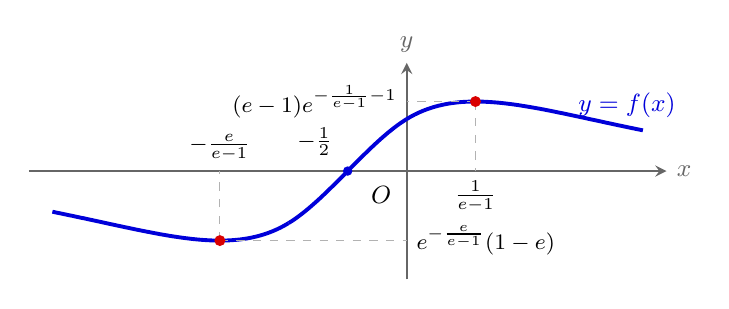
\begin{tikzpicture}[x=1.5cm, y=2.5cm, >=stealth,
    every node/.style={font=\small}]
    \coordinate (O) at (0,0);
    \draw[->, thick, gray!80!black] (-3.2,0) -- (2.2,0)
    node[right] {$x$};
    \draw[->, thick, gray!80!black] (0,-0.55) -- (0,0.55)
    node[above] {$y$};
    \node[below left=2pt] at (O) {$O$};

    % Piecewise graph of y=f(x)
    % x <= -1
    \draw[line width=1.4pt, blue!85!black, domain=-3.0:-1, samples=60]
    plot (\x, {exp(\x)*((exp(1)-1)*\x + 1)});
    % -1 <= x <= 0
    \draw[line width=1.4pt, blue!85!black, domain=-1:0, samples=40]
    plot (\x, {(1-\x)*exp(\x) - (\x+2)*exp(-\x-1)});
    % 0 <= x
    \draw[line width=1.4pt, blue!85!black, domain=0:2.0, samples=60]
    plot (\x, {exp(-\x-1)*((exp(1)-1)*\x + exp(1)-2)});

    % Key points
    \coordinate (Pmin) at ({-exp(1)/(exp(1)-1)}, {(1-exp(1))*exp(-exp(1)/(exp(1)-1))});
    \coordinate (Pmax) at ({1/(exp(1)-1)}, {(exp(1)-1)*exp(-exp(1)/(exp(1)-1))});

    % Dashed guides for minimum
    \draw[dashed, gray!60] (Pmin) -- ({-exp(1)/(exp(1)-1)}, 0);
    \node[above, font=\footnotesize] at ({-exp(1)/(exp(1)-1)}, 0) {$-\frac{e}{e-1}$};
    \draw[dashed, gray!60] (Pmin) -- (0, {(1-exp(1))*exp(-exp(1)/(exp(1)-1))});
    \node[right, font=\footnotesize] at (0, {(1-exp(1))*exp(-exp(1)/(exp(1)-1))}) {$e^{-\frac{e}{e-1}}(1-e)$};

    % Dashed guides for maximum
    \draw[dashed, gray!60] (Pmax) -- ({1/(exp(1)-1)}, 0);
    \node[below, font=\footnotesize] at ({1/(exp(1)-1)}, 0) {$\frac{1}{e-1}$};
    \draw[dashed, gray!60] (Pmax) -- (0, {(exp(1)-1)*exp(-exp(1)/(exp(1)-1))});
    \node[left, font=\footnotesize] at (0, {(exp(1)-1)*exp(-exp(1)/(exp(1)-1))}) {$(e-1)e^{-\frac{1}{e-1}-1}$};

    % Extremum points and x-intercept
    \node[circle, fill=red!85!black, inner sep=1.4pt] at (Pmin) {};
    \node[circle, fill=red!85!black, inner sep=1.4pt] at (Pmax) {};
    \node[circle, fill=blue!85!black, inner sep=1.2pt] at (-0.5,0) {};
    \node[above left=2pt, font=\footnotesize] at (-0.5,0) {$-\frac{1}{2}$};

    % Curve label
    \node[above right=3pt, blue!85!black] at (1.3,0.18) {$y=f(x)$};
  \end{tikzpicture}
  \caption{関数 $y=f(x)$ の概形}
\end{figure}

ここで$\displaystyle\lim_{x\to\infty}f(x)=0$，$\displaystyle\lim_{x\to-\infty}f(x)=0$であり，
\begin{align}
  f\left(\dfrac{-e}{e-1}\right)=e^{-\frac{e}{e-1}}(1-e)<0,\qquad
  f\left(\dfrac{1}{e-1}\right)=(e-1)e^{-\frac{1}{e-1}-1}>0
\end{align}
だから，
\begin{align}
  \begin{cases}
    \text{最大}: x=\dfrac{1}{e-1} \\
    \text{最小}: x=\dfrac{-e}{e-1}
  \end{cases}
\end{align}
である．

\end{document}
